\begin{example}[While with Two Paths]
  \label{ex:twoPathsWhile}
  %
  { \small
  \begin{figure}
  \centering
  \begin{subfigure}{.4\textwidth}
    \begin{centering}
    {\small
    $
    \begin{array}{l}
      \kw{twoPathsWhile}(n, m) \triangleq \\
    \clabel{ \assign{i}{n} }^{0} ; \\
    \clabel{ \assign{j}{0} }^{1} ; \\
        \ewhile ~ \clabel{i > 0}^{2} ~ \edo ~ \\
        \qquad \Big(
          \eif(\clabel{j < m}^{3}, \\
          \qquad \qquad \clabel{\assign{j}{j + 1}}^{4}; 
          \clabel{\assign{i}{i - 1}}^{5},\\
          \qquad \qquad \clabel{\assign{j}{0}}^{6});
          \Big)
        \end{array}
        $
    }
    \caption{}
    \end{centering}
    \end{subfigure}
  \begin{subfigure}{.5\textwidth}
    \begin{centering}
  %   \todo{abstract-cfg for two round}
  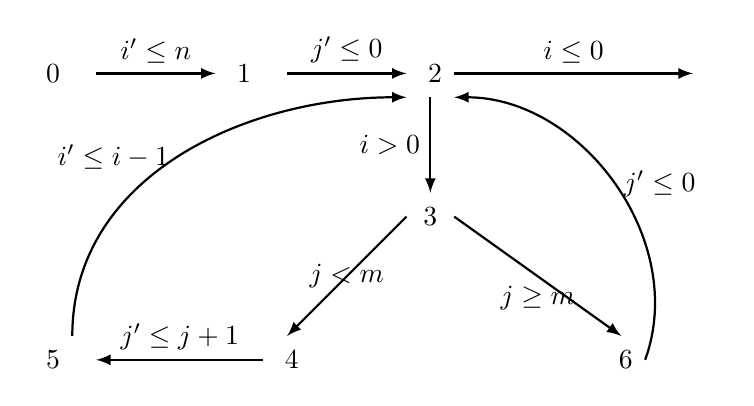
\begin{tikzpicture}[scale=\textwidth/20cm,samples=200]
  \draw[] (-8, 10) circle (0pt) node{{ $0$}};
  \draw[] (-4, 10) circle (0pt) node{{ $1$}};
  \draw[] (0, 10) circle (0pt) node{{ $2$}};
  \draw[] (0, 7) circle (0pt) node{{$3$}};
  \draw[] (-3, 4) circle (0pt) node{{ $4$}};
  \draw[] (-8, 4) circle (0pt) node{{ $5$}};
  \draw[] (4, 4) circle (0pt) node{{ $6$}};
  % Counter Variables
  \draw[] (6, 10) circle (0pt) node {\textbf{$\lex$}};
  % \draw[] (6, 4) circle (0pt) node {{ $ex$}};
  %
  % Control Flow Edges:
  \draw[ thick, -latex] (-7, 10)  -- node [above] {$i' \leq n$}(-4.5, 10);
  \draw[ thick, -latex] (-3, 10)  -- node [above] {$j' \leq 0$}(-0.5, 10);
  \draw[ thick, -latex] (0, 9.5)  -- node [left] {$i > 0$} (0, 7.5) ;
  \draw[ thick, -latex] (0.5, 7)  -- node [below] {$ j \geq m $}  (4, 4.5);
  \draw[ thick, -latex] (-7.5, 4.5)  to  [out=90,in=180]  node [left] {$i' \leq i - 1$ }(-0.5, 9.5);
  \draw[ thick, -latex] (4.5, 4)  to  [out=70,in=0]   node [right] {$j' \leq 0 $}(0.5, 9.5);
  \draw[ thick, -latex]  (-0.5, 7) -- node  {$j < m$}  (-3, 4.5) ;
  \draw[ thick, -latex]  (-3.5, 4) -- node [above] {$j' \leq j + 1$}  (-7, 4) ;
  \draw[ thick, -latex] (0.5, 10)  -- node [above] {$i \leq 0$}  (5.5, 10);
  % \draw[ thick, -latex] (6, 6.5)  -- node [right] {$\top$} (6, 4.5) ;
  \end{tikzpicture}
  \caption{}
    \end{centering}
    \end{subfigure}
  \caption{
  (a) The Two Paths While Loop Example
    (b) The Abstract Execution Control Flow Graph}
      \label{fig:twoPathsWhile}
  \end{figure}
  }
\end{example}

\begin{enumerate}
  \item  \textbf{The Abstract Control Flow Graph} is generated in Figure~\ref{fig:twoPathsWhile}(b).

  \item \textbf{Program Refinement}. 
  \\
  The \textbf{simple transition paths\footnote{For concise, the vertices sequence and the constraint for each edge in each transition path are omitted.
  The examples with sequences and annotations that are fully spelled out is in the full paper.}} are
  %  are computed as follows,
  \\
$
    \begin{array}{ll}
\tpath_0 = (0 \to 1), (1 \to 2)
&
\tpath_2 = (2 \to 3), (3 \to 6), (6 \to 2)
\\
\tpath_1 = (2 \to 3), (3 \to 4), (4 \to 5), (5 \to 2)
&
\tpath_3 = (2 \to \lex)
\end{array}
$
\\
The \textbf{repeat patterns}
for the loop that its header is
% the repeat pattern for the loop that its header is at the program point 
% loop with header 
at the program point 
$2$ are:
\\
$\rprepeat_2(\rprepeat_1(\tpath_1); \tpath_2) $
and $\rprepeat_1(\tpath_1)$; 
\\
The \textbf{refined program\footnote{$\rprog$ is used as the inputs (/ arguments) of the computations in the following steps.
For concise, it is omitted since all the arguments in the following computations are referring to the same $\rprog$.}} is
\\
$
  \tpath_0 ; \rpchoose{2: \rprepeat_2(\rprepeat_1(\tpath_1); \tpath_2) , 
  2: \rprepeat_1(\tpath_1) }; \tpath_3
$
\item \textbf{Ranking Function Computation}:
\\
  The \textbf{ranking function / (local bound)}  assigned to each edge is as follows,
    \\  
      $\locbound(0 \to 1) = 1$ 
      \quad
      $\locbound(1 \to 2) = 1$ 
      \quad
      $\locbound(2 \to \lex) = 1$ 
      \quad $\locbound(2 \to 3) = i$ 
      \quad $\locbound(3 \to 6) = i$ 
      \quad $\locbound(3 \to 4) = i$ 
      \quad $\locbound(4 \to 5) = i$ 
      \quad $\locbound(5 \to 2) = i$ 
      \quad $\locbound(6 \to 2) = i$ 
      \\
  The bound on the maximum value of the ranking function $i$, i.e., the \textbf{ranking function bound} is
    $\varinvar(i) = n$.
    \\
    The \textbf{path-insensitive transition bound} for each edge:
    \\  
      $\absclr(0 \to 1) = 1$
      \quad $\absclr(1 \to 2) = 1$
      \quad $\absclr(2 \to \lex) = 1$ 
      \quad $\absclr(2 \to 3) = n$ 
      \quad $\absclr(3 \to 6) = n$ 
      \\
      \quad $\absclr(3 \to 4) = n$ 
      \quad $\absclr(4 \to 5) = n$ 
      \quad $\absclr(5 \to 2) = n$ 
      \quad $\absclr(6 \to 2) = n$ 
  % \\
  % $\bot$ means the algorithm fails in inferring the ranking bound.
  \item \textbf{Outside-In Algorithm}:\\
  The \textbf{Outside-In} bound for every $\rpattern$ w.r.t. the refined program $\rprog$ is as follows,
  \[
    \begin{array}{l}
        \outinB(\tpath_0) = 1
        \\
        \outinB(2: \rprepeat_1(\tpath_1)) = m 
        \\
        \outinB(2: \rprepeat_2(\rprepeat_1(\tpath_1); \tpath_2)) = \lfloor\frac{n}{m}\rfloor
        % \\
        % \outinB(\rpchoose{\rprepeat_2(\rprepeat_1(\tpath_1); \tpath_2), \rprepeat_1(\tpath_1) })
        % = \max\{m, (m  + 1)\times \lfloor\frac{n}{m}\rfloor\}
\end{array}
\]
\item \textbf{Inside-Out Algorithm}
\begin{itemize}
  \item \textbf{Repeat Chain Set}
  \\
  $\rpchset(2, \tpath_1) = \{\rprepeat_1(\tpath_1) \to \tpath_1, \rprepeat_2(\rprepeat_1(\tpath_1); \tpath_2) \to \rprepeat_1(\tpath_1) \to \tpath_1\}$ \\
  $\rpchset(2, \tpath_2) = \{\rprepeat_2(\rprepeat_1(\tpath_1); \tpath_2) \to  \tpath_2\}$ \\
  $\rpchset(\_, \_) = \emptyset$ 
  % \\
  \item \textbf{Repeat Chain Bound}
  %  for every simple transition path $\tpath$ through its \emph{Repeat Chain}s
  \\
  $\rpchB(2, \tpath_1) = \max\{m, m \times \lfloor\frac{n}{m}\rfloor\}$ \\
  $\rpchB(2, \tpath_2) = \lfloor\frac{n}{m}\rfloor$ 
  %
  \item \textbf{Loop Chain}
  \\
  $\lpch(\tpath_0) = \tpath_0$ \qquad
  $\lpch(\tpath_1) = 2\to \tpath_1$ \\
  $\lpch(\tpath_3) = \tpath_3$ \qquad
  $\lpch(\tpath_2) = 2\to \tpath_2$ 
  \item \textbf{{Relative Loop Bound}}
  %  for every simple transition path $\tpath$ through its \emph{Loop Chain}
  \\
  $\rpchB(2, \tpath_1) = \max\{m, m \times \lfloor\frac{n}{m}\rfloor\}$ \quad
  $\rpchB(2, \tpath_2) = \lfloor\frac{n}{m}\rfloor$  \\
  $\rpchB(\bot, \tpath_0) = 1$ \quad
  $\rpchB(\bot, \tpath_3) = 1$ 
  \item \textbf{Inside-Out Bound}
  \\
  $\inoutB(\tpath_1) = n$ \quad
  $\inoutB(\tpath_2) = \lfloor\frac{n}{m}\rfloor$ \quad
  $\inoutB(\tpath_0) = 1$ \quad
  $\inoutB(\tpath_3) = 1$ 
\end{itemize}
\item \textbf{Path-sensitive Reachability-Bound} on every program control location
\\
$\psRB(0) = \psRB(1) = \psRB(\lex) = 1$ \qquad
$\psRB(4) = \psRB(5) = \max\{m, m \times \lfloor\frac{n}{m}\rfloor\}$ 
\\
$\psRB(3) = \psRB(2) = \max\{m, m \times \lfloor\frac{n}{m}\rfloor\} + \lfloor\frac{n}{m}\rfloor + 1 $
\quad $\psRB(6) = \lfloor\frac{n}{m}\rfloor$ 
% $\psRB(\{0, 1, \lex\}) = 1$ \qquad
% $\psRB(\{6 \}) = \lfloor\frac{n}{m}\rfloor$ \\
% $\psRB(\{4, 5 \}) = \max\{m, m \times \lfloor\frac{n}{m}\rfloor\}$ \quad
% $\psRB(\{3, 2 \}) = \max\{m, m \times \lfloor\frac{n}{m}\rfloor\} + \lfloor\frac{n}{m}\rfloor + 1 $ \\
\end{enumerate}